\chapter{Archimedes' Principle}

\section{Aim}
To investigate the relationship between the weight of the fluid displaced by a body and upthrust

\section{Background Information}
When a body is placed in a fluid it experiences an upward force (Upthrust) from the fluid. This force enables the object to float or seem lighter when it is placed into the fluid. Thus, swimming and flotation of bodies depend on this upthrust. 

Whenever a body is partially or totally immersed in a fluid it tends to displace some of the fluid. Therefore, there might be a relationship between upthrust and the weight of the fluid displaced. 

\section{Materials}
Eureka can, beaker, beam balance, Spring balance, Measuring cylinder, Retort stand, stone, thread and water.

\section{Procedure}
\begin{enumerate}
\item Measure the mass of an empty measuring cylinder by using a beam balance and record it as $m_1$.
\item Clamp a spring balance onto a retort stand then tie a stone with a thread and suspend it on the hook of the spring balance. Read and record the \textit{weight} of the stone suspended in air as $w_1$.
\item Fill the Eureka can with water until some water overflows from the spout into a beaker placed below the spout. Wait until the overflowing water stops.  
\item  Remove the beaker and instead place a measuring cylinder. Lower the stone into the Eureka can while it is still suspended on the spring balance until the stone is submerged in water. Make sure the stone does not touch the bottom or the sides of the Eureka can.  
\item Wait until no more water flows out of the spout then read on the spring balance the weight of the stone submerged in the water and record it as $w_2$.
\item Measure the mass of the measuring cylinder with the collected water and record it as $m_2$.
\end{enumerate}

\begin{figure}[h!]
\centering
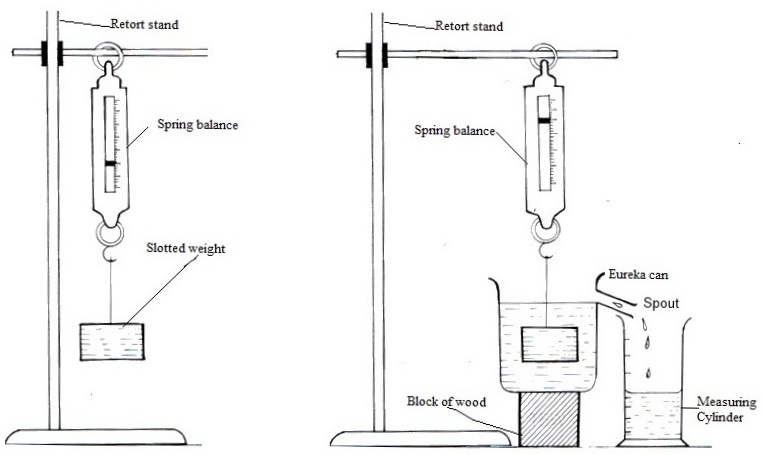
\includegraphics[width=13cm]{./img/archimedes-1.jpg}
\caption{Archimedes' Principle practical setup}
\label{fig:archimedes-1}
\end{figure}

\section{Analysis and Interpretation}
\begin{enumerate}
\item What is the mass of the water collected?
\item Find the weight of water collected, label it $w_d$.
\item Find the difference between $w_1$ and $w_2$, and label it $w_L$. What does this value represent? What is the cause of this difference in the weight of the stone? 
\item Compare the values of $w_L$ and $w_d$.
\end{enumerate}

\section{Conclusion}
From the experiment, how is the upthrust related to the weight of the fluid displaced?

\section{Questions for Discussion}
\begin{enumerate}
\item Why should the stone not touch the bottom or sides of the Eureka can during the experiment?
\item How are the final results affected by your measurements during the experiment?
\item Can this experiment be used to determine the relative density of an object? Explain.
\end{enumerate}

\section{Reflection and Self Assessment}
\begin{enumerate}
\item Is there anything in this experiment you do not understand? If so, what is it, and in what ways could you increase your understanding?
\item Which part of the experiment was interesting to you and which part was not interesting? Explain.
\item What problems did you face in this experiment and how could you solve them next time?
\item How can you use what you have learned in this experiment in everyday life?

\end{enumerate}